\definition{The \b{chain rule} computes the derivatives for \b{compositions} of functions \f{g(x)} and \f{f(y)=f(g(x))=z} as:
\cf{
    (f\circ g)^\prime(x) = (f(g(x)))^\prime = f^\prime(g(x))\cdot g^\prime(x)
}
\cf{
    \frac{\delta z}{\delta x} = \frac{\delta z}{\delta y}\frac{\delta y}{\delta x} = \frac{\delta f(g(x))}{\delta g(x)}\frac{\delta g(x)}{\delta x}
}}

Generalizing this formulation to the multidimensional case with leads us to:

\cf{
    \frac{\delta z}{\delta x_i}=\sum_{j}^{}\frac{\delta z}{\delta y_j}\frac{\delta y_j}{\delta x_i}
}
where \f{x\in\mathbb{R}^m, y\in\mathbb{R}^n, g:\mathbb{R}^m\to\mathbb{R}^n, f:\mathbb{R}^n\to\mathbb{R}} and \f{y = g(x)} and \f{z = f(y)}. Transforming this formulation into vector notation gives us:
\cf{
    \nabla_{x}z=(\frac{\delta y}{\delta x})^T\nabla_yz,
}
where \f{\frac{\delta y}{\delta x}} is the \f{n\times m} Jacobian matrix of \f{g}, and \f{\nabla_yz} being the gradient of z with respect to vector \f{y}. Since \f{y \in \mathbb{R}^n} this leaves us with:
\cf{
    \nabla_yz=\left[ \frac{\delta z}{\delta y_1}, \frac{\delta z}{\delta y_2}, ..., \frac{\delta z}{\delta y_n} \right]^T
}

\subsection{Derivations of Activations}
\begin{itemize}
    \item \b{Linear:} \f{h^\prime(z)=1}
    \item \b{Sigmoid:} \f{h^\prime(z)=h(z)(1-h(z))}
    \item \b{Tanh:} \f{h^\prime(z)=1-h(z)^2}
    \item \b{ReLU:} \f{h^\prime(z)=\begin{cases}
        1, z>0\\
        0, z\leq0
    \end{cases}}
\end{itemize}

\subsection{Backpropagation in Neural Networks}
\vspace{0.3cm}
\begin{figure}[h]
    \centering
    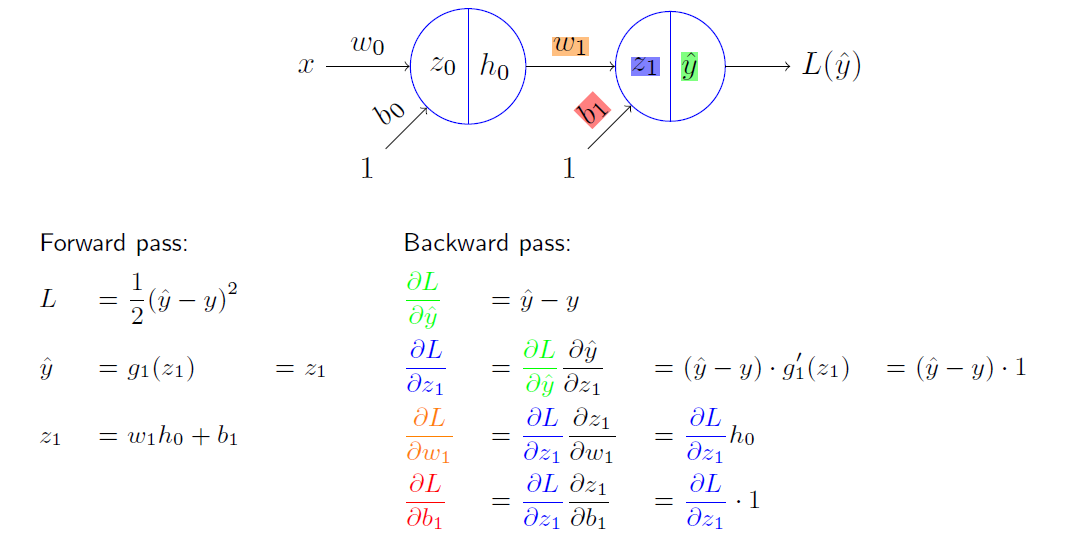
\includegraphics[width=0.9\textwidth]{bp1.png}
\end{figure}
\vspace{0.3cm}
\begin{figure}[h]
    \centering
    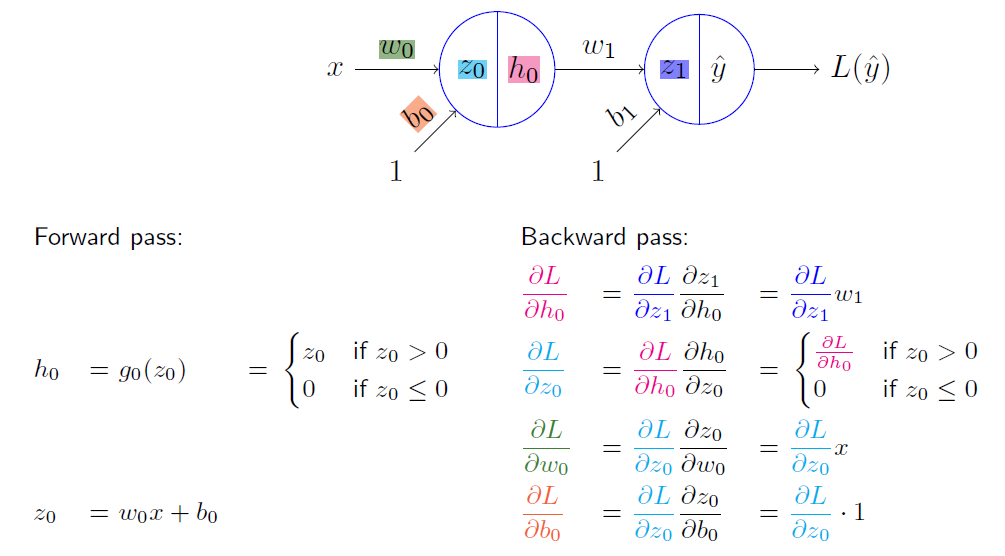
\includegraphics[width=0.9\textwidth]{bp2.png}
\end{figure}

\b{Note:} The gradient of a skip connection is computed by summing the incoming derivatives of both the forward and skip connection.